\documentclass[12pt,letterpaper]{article}
\usepackage[utf8]{inputenc}
\usepackage{amsmath}
\usepackage{amsfonts}
\usepackage{amssymb}
\usepackage{multirow}
\usepackage{longtable}
\usepackage{graphicx}
\title{DND Inventory System Plan}
\date{January 11, 2020}

\begin{document}
	\begin{titlepage}
		\maketitle
		\begin{center}
		\end{center}
			
		
		\thispagestyle{empty}
		\pagebreak
	\end{titlepage}

	\section{Project Overview}
		\subsection{Project Goal}
			\paragraph{\indent Project \emph{DND Inventory System} will allow users to track and dynamically alter one or more of the user's character's inventory and currently equipped items, affecting character's stats as a result.}
		\subsection{Scope of Work}
			\paragraph{\indent Kasin Sparks will perform all of the following task to the best of their abilities:}
			\begin{enumerate}
				\item Server partition creation and management*
				\begin{enumerate}
					\item Server partition will be subject to the following terms
					\begin{itemize}
					\item Partition size equal to 10 gigabytes (where 1 gigabyte = 1000 megabytes) worth of storage space. 
					\item Upload and Download speeds limited by Upload and Download speed provided by Internet Service Provider (ISP) 
					\end{itemize}
					\item Management will include the following:
					\begin{itemize}
						\item Online or over the phone assistance. Monday through Fridays from 9a.m. to 6p.m. EST.
						\item Assistance with service migration to another server. 
						\item Minimum of ONE year (365 days) of server support, that will end 365 days after product is delivered to client, with optional renewal of support per year.
					\end{itemize}
				\end{enumerate} 
				\item Web app creation
					\begin{enumerate}
						\item Flask application
						\item SQLite3 database
						\item Front end HTML, CSS, JavaScript, and Asynchronous JavaScript And XML (AJAX) to standards agreed upon.			
					\end{enumerate}
			\end{enumerate} 
			* Only valid if Kasin Sparks is able to have ports 80/433 open via Internet Service Provider (ISP) and if ISP allows such services.\\
			\paragraph{\indent Client's Responsibility}
			\begin{enumerate}
				\item Provide Kasin Sparks with all necessary assets.
				\item Willing and able to assist Kasin Sparks with knowledge and mechanics relating to inventory system.	
			\end{enumerate}
		\subsection{Project Timeline}
			\begin{table}[hbt]
				\begin{tabular}{|l|l|}
					\hline
					\multicolumn{1}{|c|}{Task} & \multicolumn{1}{|c|}{Period} \\ \hline
					Server Allocation & Month XX, 2020 - Month XX, 2020 \\ \hline
					SQLite3 Database Creation and Setup & Month XX, 2020 - Month XX, 2020 \\ \hline
					Flask Application Creation & Month XX, 2020 - Month XX, 2020 \\ \hline
					Front End Creation & Month XX, 2020 - Month XX, 2020 \\ \hline
					\bf{Target First Round Review*} & \bf{Month XX, 2020} \\ \hline
					\bf{Target Delivery Date} & \bf{Month XX, 2020} \\ \hline
				\end{tabular}
				\caption{Proposed Project Timeline}
				\label{tab:tableProjectTimeline}
			\end{table}
			\paragraph{\indent *After \emph{Target First Round Review}, the timeline will be assessed. If work that was not listed in agreed upon plan is needed, an updated schedule will be attached in the Addendum.\\}
	\section{Front End}
		\subsection{Character/Inventory}
		\paragraph{\indent Figure \ref{fig:markedUpMockup} and \ref{fig:mockup} show the planed layout of the application*. Group name will include, but not limited to, Armour, Weapons, etc. Groups may have subgroups that will also be collapsible. }
		\paragraph{\indent Main menu screen is not shown.}
		* Layout is subject to change.
	\section{Back End}
		\subsection{Programming Stack}
			\paragraph{\indent The programming stack for project \emph{DND Inventory System} will include the following technologies: }
				\begin{description}
					\item[Linux] Ubuntu 18.04.03 LTS will be the flavor of Linux used for server operating system. For more information about Ubuntu, please visit \emph{https://ubuntu.com}\\
					\item[Apache2] Web server that will be used on the server to handle serving the website. Please visit \emph{https://httpd.apache.org/} for more information about Apache2.\\
					\item[SQLite3] will be leveraged for the database and will be used to store all data pertaining to the users and website. For information regarding user data please see Table \ref{tab:tableUserData}. Please visit \emph{https://sqlite.org/index.html} for more information about SQLite3.\\
					\item[Flask] a web application framework which uses python, Werkzeug, and Jinja. Flask will be used to handle the back-end operations such as, but not limited to, communication to database, dynamic web page generation, user handling, business logic. Please visit \emph{https://pypi.org/project/Flask} for more information.\\
					\item[Docker] will be used to containerize the application which will in turn make the app more shareable and deployable. For more information, please visit \emph{https://www.docker.com}\\ 
				\end{description}  
		\subsection{Data}
			\paragraph{\indent Tables \ref{tab:tableUserData}, \ref{tab:tableInventory}, \ref{tab:tableCharaterData}, and \ref{tab:tableCharacterEquipment} details data fields and data descriptions that will be used in the Web-app. Data may be represented differently in database, but will contain the fields as shown. \\}
			\paragraph{\indent User's username and password will be hashed using an Advanced Encryption Standard (AES). \\}

			
	\clearpage

	\section{Tables and Figures}
	\begin{figure}[hbt]
		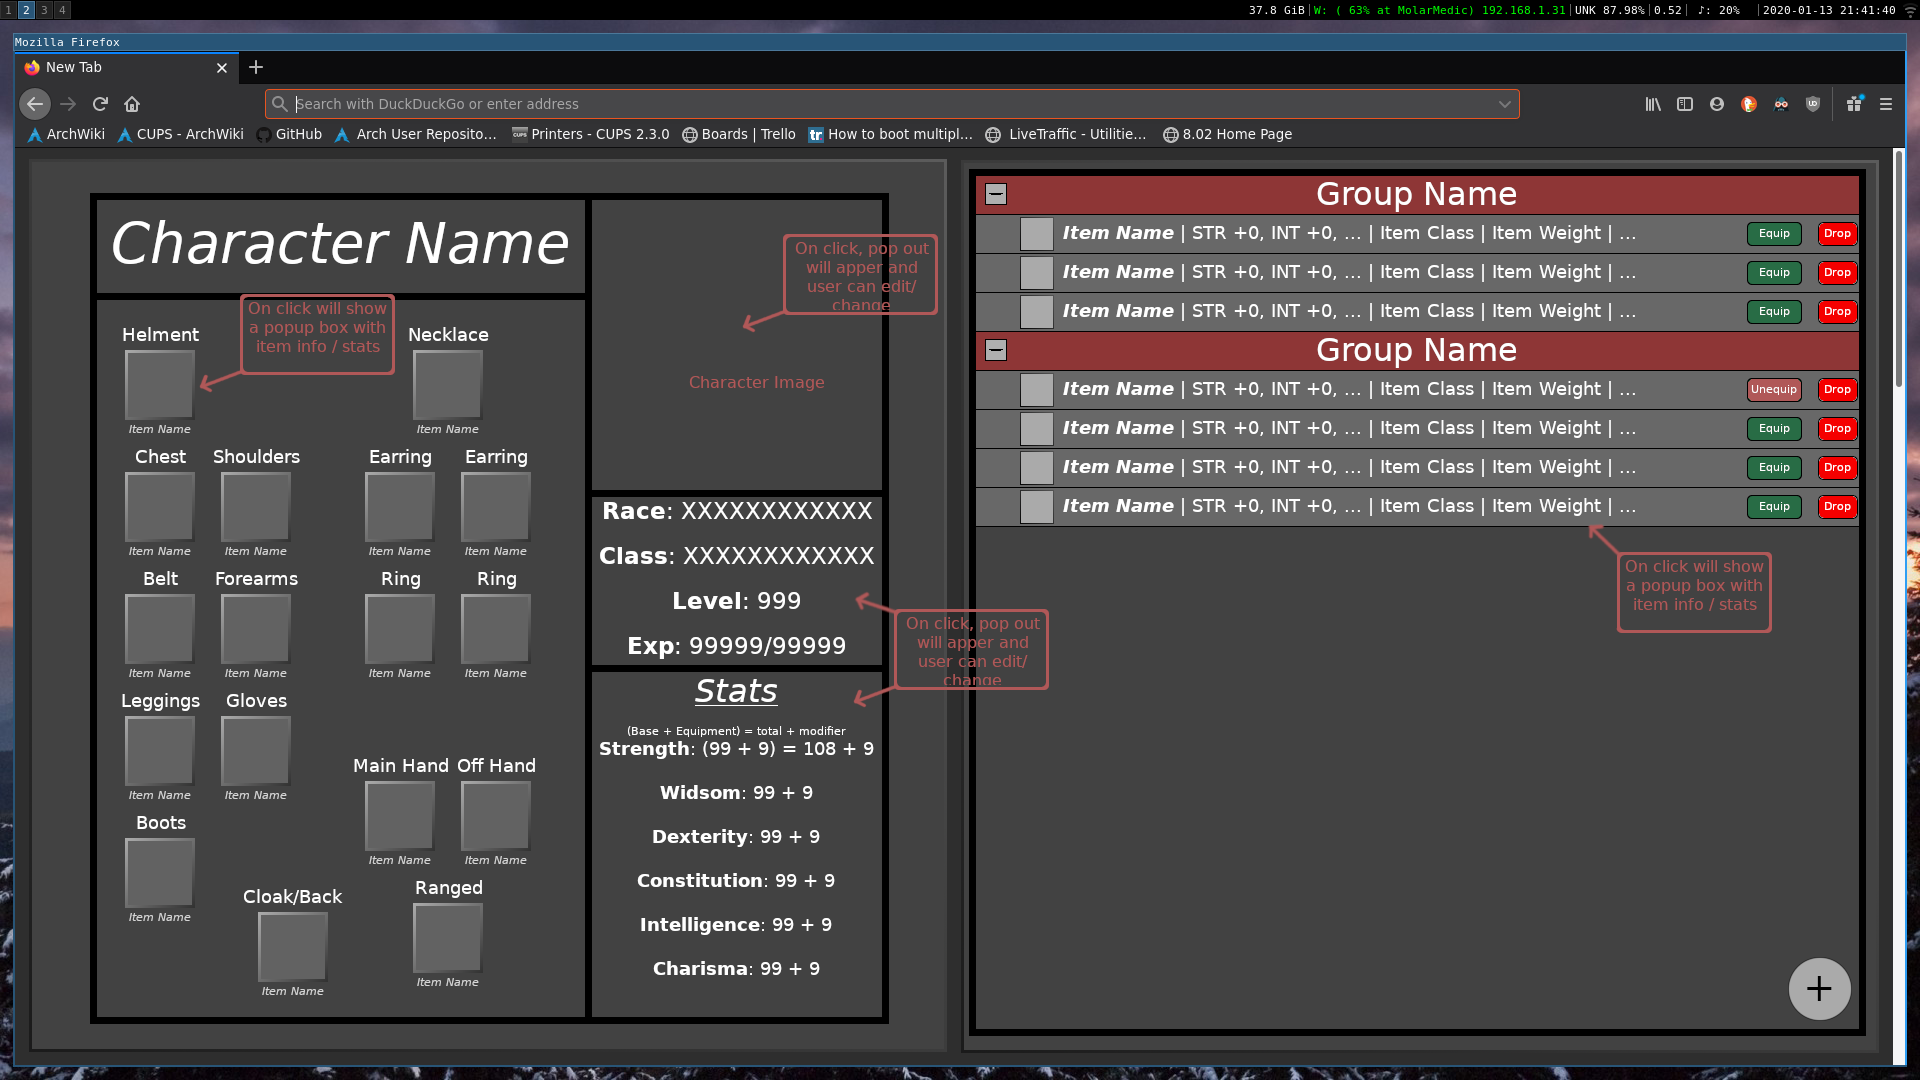
\includegraphics[width=\linewidth]{Second_Mockup_Anotated.png}		
		\caption{Mock up}
		\label{fig:markedUpMockup}
	\end{figure}

	\begin{figure}[hbt]
		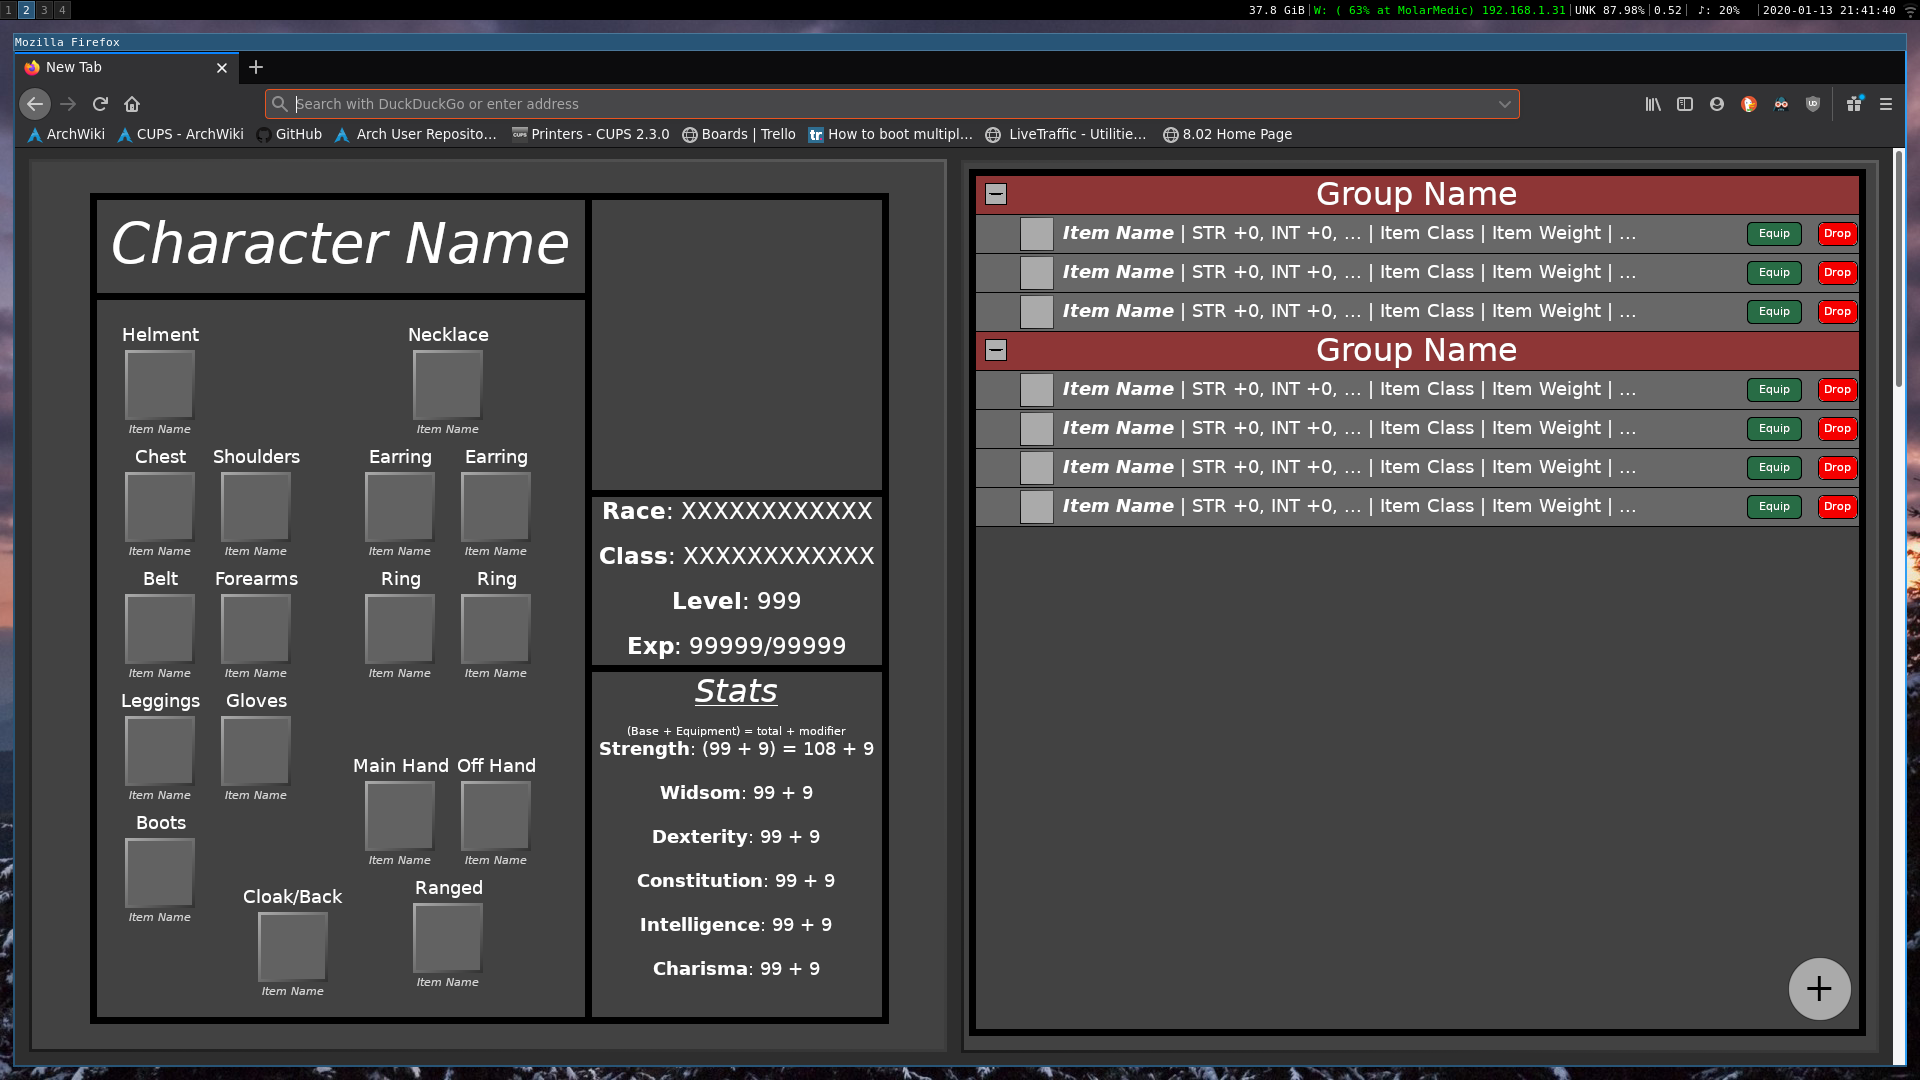
\includegraphics[width=\linewidth]{Second_Mockup.png}		
		\caption{Mock up}
		\label{fig:mockup}
	\end{figure}


	\begin{table}[h]
		\centering
		\begin{tabular}{| l | l | p{7cm} |}
			\hline
			\multicolumn{1}{|c|}{\bf{Field}} & \multicolumn{1}{|c|}{\bf{Data Type}} & \multicolumn{1}{|c|}{\bf{Description}}\\ \hline
			User ID & Integer & User will be assigned an integer upon sign-up. For internal use only \\ \hline
			Username & String & User's hashed login name \\ \hline
			Display Name & String & User's name that will be visible to the user \\ \hline
			Password & String & User's hashed password \\ \hline 
		\end{tabular}
		\caption{User Data}
		\label{tab:tableUserData}
	\end{table}			

	\begin{table}[h]
		\centering
		\begin{tabular}{| l | l | p{7cm} |}
			\hline
			\multicolumn{1}{|c|}{\bf{Field}} & \multicolumn{1}{|c|}{\bf{Data Type}} & \multicolumn{1}{|c|}{\bf{Description}}\\ \hline
			Inventory & Item & User's character inventory. Item will be a custom data type. \\ \hline
		\end{tabular}
		\caption{Inventory}
		\label{tab:tableInventory}
	\end{table}			
	
	\begin{table}[h]
		\centering
		\begin{tabular}{| l | l | p{7cm} |}
			\hline
			\multicolumn{1}{|c|}{\bf{Field}} & \multicolumn{1}{|c|}{\bf{Data Type}} & \multicolumn{1}{|c|}{\bf{Description}}\\ \hline
			Character ID & Integer & Track user's characters. For internal use only \\ \hline
			Character Name & String & User's character name \\ \hline
			Class & String & Character's class \\ \hline
			Race & String & Character's race \\ \hline
			Level & Integer & Character's level \\ \hline
			Current Experience & Integer & Character's current experience level \\ \hline
			Max Level Experience & Integer & The number of experience points needed to next level \\ \hline
			Strength & Integer & Character's strength \\ \hline
			Dexterity & Integer & Character's dexterity \\ \hline
			Constitution & Integer & Character's constitution \\ \hline
			Intelligence & Integer & Character's intelligence \\ \hline
			Wisdom & Integer & Character's wisdom \\ \hline
			Charisma & Integer & Character's charisma \\ \hline
			... & ... & ... \\ \hline
			\hline

		\end{tabular}
		\caption{Character Data}
		\label{tab:tableCharaterData}
	\end{table}			

	\begin{table}[h]
		\centering
		\begin{tabular}{| l | l | p{7cm} |}
			\hline
			\multicolumn{1}{|c|}{\bf{Field}} & \multicolumn{1}{|c|}{\bf{Data Type}} & \multicolumn{1}{|c|}{\bf{Description}}\\ \hline
			Helmet & Item & \\ \hline
			Chest Piece & Item & \\ \hline
			Shoulders & Item & \\ \hline
			Forearms & Item & \\ \hline
			Gloves & Item & \\ \hline
			Leggings & Item & \\ \hline
			Boots & Item & \\ \hline
			Main Hand & Item & \\ \hline
			Off Hand & Item & \\ \hline
			Ring Slot 0-9 & Item & \\ \hline
			... & ... & \\ \hline
		\end{tabular}
		\caption{Character's Equipment}
		\label{tab:tableCharacterEquipment}
	\end{table}			

	\begin{table}[h]
		\begin{tabular}{| l | l | p{7cm} |}
			\hline
			\multicolumn{1}{|c|}{\bf{Field}} & \multicolumn{1}{|c|}{\bf{Data Type}} & \multicolumn{1}{|c|}{\bf{Description}}\\ \hline
			ID & Integer & \\ \hline
			Picture & Image & \\ \hline
			Item Name & String & \\ \hline
			Item Description & String & \\ \hline
			Item Level & Integer & \\ \hline
			Item Class & String & \\ \hline
			Item Slot & String & \\ \hline
			Strength Bonus & Integer & \\ \hline
			Dexterity Bonus & Integer & \\ \hline
			Constitution Bonus & Integer & \\ \hline
			Intelligence Bonus & Integer & \\ \hline
			Wisdom Bonus & Integer & \\ \hline
			Charisma Bonus & Integer & \\ \hline
			... & ... & \\ \hline
			
		\end{tabular}
		\caption{Item}	
		\label{tab:tableItem}
	\end{table}


\end{document}